\documentclass{report}

\title{ Software Engineering Theory and Practice}
\makeatletter
\renewcommand\@date{{%
		\vspace{-4em}%
		\large\centering
		\begin{tabular}{@{}c@{}}
			Yusuf A. \\
			\normalsize yusufa42@hotmail.com
			\bigskip \bigskip 
			\\ \today
		\end{tabular}%
}}
\makeatother

\usepackage{listings}
\usepackage{xcolor}
\usepackage{parskip}
\usepackage{graphicx}
\usepackage{subfig}
\usepackage{fancyvrb}
\usepackage{color}  
\usepackage{hyperref}
\graphicspath{ {img/} }

\hypersetup{
	colorlinks=true, 
	linktoc=all,    
	linkcolor=blue,  
}

\definecolor{codegreen}{rgb}{0,0.6,0}
\definecolor{codegray}{rgb}{0.5,0.5,0.5}
\definecolor{codepurple}{rgb}{0.58,0,0.82}
\definecolor{backcolour}{rgb}{0.95,0.95,0.92}

\lstdefinestyle{code}{
	backgroundcolor=\color{backcolour},   
	commentstyle=\color{codegreen},
	keywordstyle=\color{magenta},
	numberstyle=\tiny\color{codegray},
	stringstyle=\color{codepurple},
	basicstyle=\ttfamily\footnotesize,
	breakatwhitespace=false,         
	breaklines=true,                 
	captionpos=b,                    
	keepspaces=true,                 
	numbers=left,                    
	numbersep=5pt,                  
	showspaces=false,                
	showstringspaces=false,
	showtabs=false,                  
	tabsize=2
}

\lstset{style=code}

\begin{document}
	\maketitle
	\tableofcontents
	\newpage
	
	\section{Problem Specification}
	
	\subsection{Analysing the competition and extracting key points}
	
	I have chosen two project management applications, Jira and Trello, to use as anchors for my problem specification.
	Problems that arise from using both applications include overwhelming complexity, large configuration overhead,
	and creating strain on physical resources.
	
	\subsection{Trello: simple, accessible, but less applicable}
	
	Trello excels over Jira due to its more prominent focus on being friendlier towards user accessibility, through having
	a simpler interface and better cross-platform compatibility. On the same note, Trello falls short of its capability to meet
	more complex project management goals compared to Jira due to its lesser customisability.
	
	\subsection{Jira: robust, scalable, but more complex}
	
	Jira enjoys a wider and more scalable ecosystem to meet the demands of a growingly more complex management
	solution, albeit lending itself more towards the software development field as it supports more features tailored towards
	a technically-oriented design goal, by means of reporting and analytics, bug/issue tracking, external integration, etc.
	
	\subsection{Collating the criteria for a successful project management application}
	
	Trello and Jira share similarities in robustness and applicability to most situations that an individual, or small team
	of people would need to co-ordinate a successful project to its end. If we were to target this audience, simply the
	core principles of robustness, visual simplicity,  intuitive interfaces and narrow initial learning curve are what make
	these applications fundamentally fit for purpose.
	
	Trello is the most natural source to gather requirements from based on my target audience, because it leans more
	towards catering for smaller projects, and focuses on being easier to access, opposed to overwhelming for the price
	of meticulous management.
	
	\subsection{Developing the user requirements based off the criteria specified}
	
	With the core principles of robustness, simplicity and generality in mind, my specifications for the proposed project
	management solution are as follows:
	
	\begin{enumerate}
		\item \textbf{Stability:} The system should be stable, in so meaning that in the worst case, it should never affect
				 the databases involved, nor any user-provided information, and it should be capable of recovering its
				 own state.
		\item \textbf{Usability:} The interface should be intuitive, and any features should be easily accessible, or in some
				  capacity be capable of being intuited by the user. Prominent features should be readily available with a few
				  mouse clicks.
		\item \textbf{Security:} Confidential user-provided data should be stored securely, and room should be left for
				  extensibility later down the road. Proper security standards should be adhered to, and where not,
				  supplemental software should be allowed to to integrate easily.
	\end{enumerate}
	
	\subsection{Developing the system requirements}
	
	Notably from Trello, the core ideas relevant to the system requirements regard perceived ease-of-use, accessibility,
	and quickly starting from nothing into a fully fledged solution:
	
	\begin{enumerate}
		\item \textbf{Performance:} Relatively large datasets should be manageable for the targeted audience's physical
				  specifications, without incurring noticeable input delay or responsiveness.
		\item \textbf{Cross-compatibility:} Accessibility between different operating systems is essential for reaching a
				  larger market share, and allowing diverse teams to work together.
		\item \textbf{Configuration:} Allowing flexibility in the configuration to accommodate different platform setups
				  is essential to minimising the initial burden which most commercial project management solutions face.
	\end{enumerate}
	
	Additionally, to ensure that development is retraceable and scalable, the project will be versioned using 
	\verb|git| to track changes, bugs, and any potential branching for larger implementations down the road.
	
	\newpage
	\section{Design}
	
	\subsection{Describing and modeling the system’s architecture}
	\vspace{1em}
	\begin{figure}[h]
		\centering
		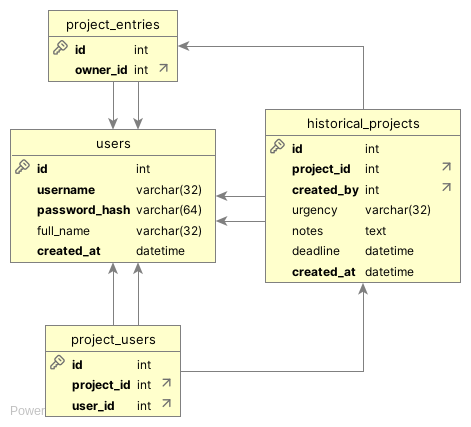
\includegraphics[width=0.5\textwidth]{overview}
		\caption{High-level architectural view}
	\end{figure}
	\vspace{1em}
	A user system is implemented to attribute projects and revisions to an individual user. Historical projects (or revisions)
	are frozen versions of a project after a certain change has been applied by either the owner, or a user who is 
	on the \verb|project_users| association:
	\vspace{1.5em}
	\begin{lstlisting}[language=Python]
		class HistoricalProject(Base):
			__tablename__ = 'historical_projects'
			
			id: Mapped[int] = mapped_column(Integer, primary_key=True)
			project_id: Mapped[int] = mapped_column(
				Integer, ForeignKey('project_entries.id'), nullable=False
			)
			created_by: Mapped[int] = mapped_column(
				Integer, ForeignKey('users.id'), nullable=False
			)
			urgency: Mapped[str] = mapped_column(
				String(32), nullable=True
			)
			notes: Mapped[Text] = mapped_column(Text(), nullable=True)
			deadline: Mapped[DateTime] = mapped_column(
				DateTime, nullable=True
			)
			project_users: Mapped[list["ProjectUser"]] = relationship(
				"ProjectUser",
				primaryjoin=\
					"HistoricalProject.id == ProjectUser.project_id",
				lazy="subquery",
				cascade="all, delete-orphan"
			)
			created_at: Mapped[DateTime] = mapped_column(
				DateTime(timezone=True), server_default=func.now()
			)
	\end{lstlisting}
	\vspace{1.5em}
	As it is, when a project is created by a registered user, there is no "project" created, it simply creates an initial
	revision which is tied to the creating user and a \verb|ProjectEntry| association.
	Any time that a project is modified in any way whatsoever by the end user, a corresponding \verb|HistoricalProject|
	is appended. This architectural decision promotes robust management of changes and "replay-ability", meaning
	that a project can be able to be reconstructed and/or rolled back to an older state.
	
	Although users are represented equally, with no role system existing, the system acknowledges the difference
	between a project creator and a project user, and so affords the creator more permissions, i.e. being able to
	outright delete selected revisions (unless it is the last one existing.)
	
	\subsection{Describing the system's usability, security and performance}
	
	The system is written in \verb|Python|, a programming language that has great support for UI development
	needs with little set-up time. The UI library itself is \verb|Qt5| developed by \verb|the Qt Company|, which is
	a commonly used, cross-platform and highly performant library.
	
	\subsubsection{Usability}
	
	The program is split into two primary forms: the registration/login, and the primary form.
	\vspace{1em}
	\begin{figure}[h]
		\centering
		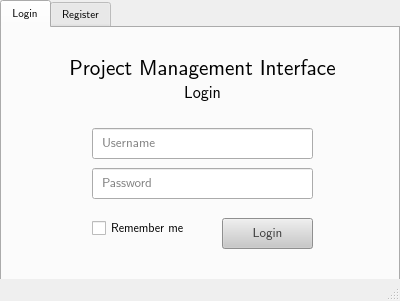
\includegraphics[width=5cm]{login}
		\qquad
		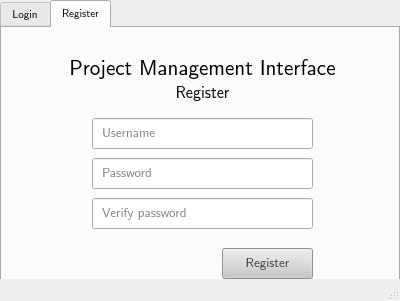
\includegraphics[width=5cm]{register}
		\caption{Login/registration}
	\end{figure}
	Both forms employ a tab system in one way or another to avoid extraneous gymnastics for the user, and
	keep everything confined to one window unless absolutely necessary.
	
	\begin{figure}[h]
		\centering
		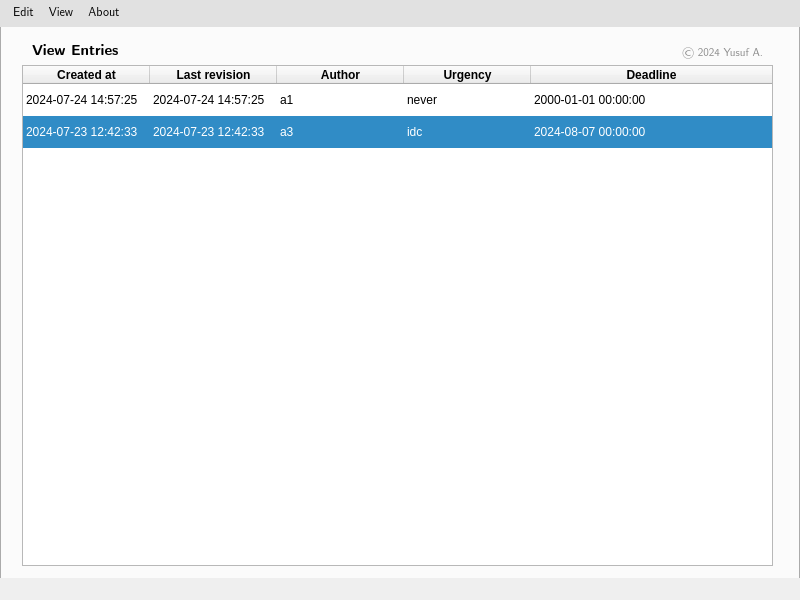
\includegraphics[width=0.7\textwidth]{view-entries}
		\caption{High-level architectural view}
		\label{fig:view_entries}
	\end{figure}
	
	The \verb|View Entries| view (Fig. \ref{fig:view_entries}) is displayed after logging in manually, or automatically
	(via saved credentials), everything is accessible to the user through the action bar. The \verb|Help| view explains
	how to navigate projects and revisions (in Fig. \ref{fig:help}), this is available under the \verb|About| action, as
	would be expected on any other similar program.

	\begin{figure}[h]
		\centering
		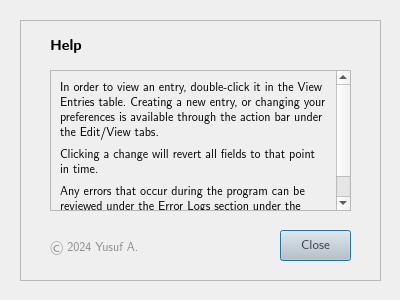
\includegraphics[width=0.6\textwidth]{help}
		\caption{Help view}
		\label{fig:help}
	\end{figure}
	
	When deciding to create a new project under the \verb|Edit| $\rightarrow$ \verb|Create new entry| action, the
	user is able to simply create a new project, assign project users, and be automatically routed to the
	\verb|View/Edit Entries| form upon creation, as displayed in Fig. \ref{fig:edit-entry}.

	\begin{figure}[h]
		\centering
		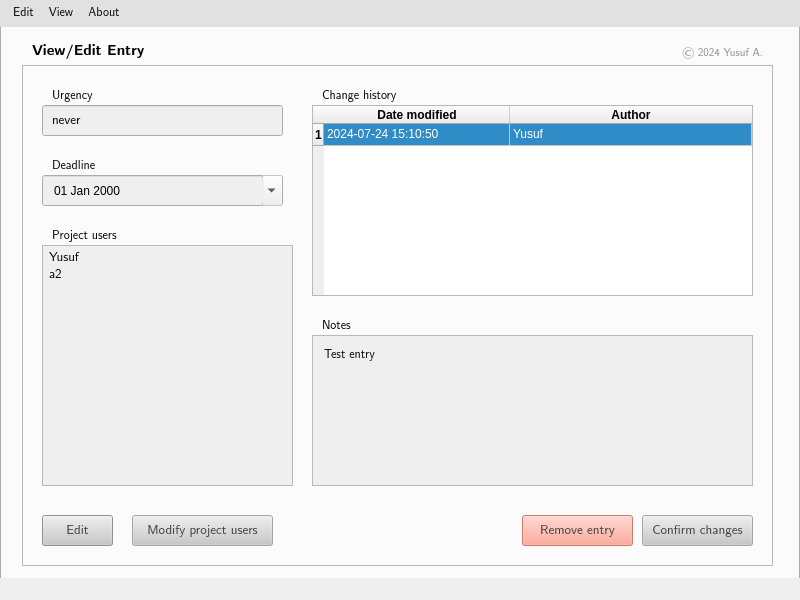
\includegraphics[width=0.8\textwidth]{edit-entry}
		\caption{View/edit entries}
		\label{fig:edit-entry}
	\end{figure}
	
	From here, toggling the \verb|Edit| button will enable write access to any properties of the project, and upon
	committing the changes with \verb|Confirm changes|, will create a new revision that is automatically selected
	in the change history table. Any user will be able to view these revisions by selecting them, however unless
	they are on the latest version's \verb|Project users| list, they will not be able to edit any aspect of the project.

	\begin{figure}[h]
		\centering
		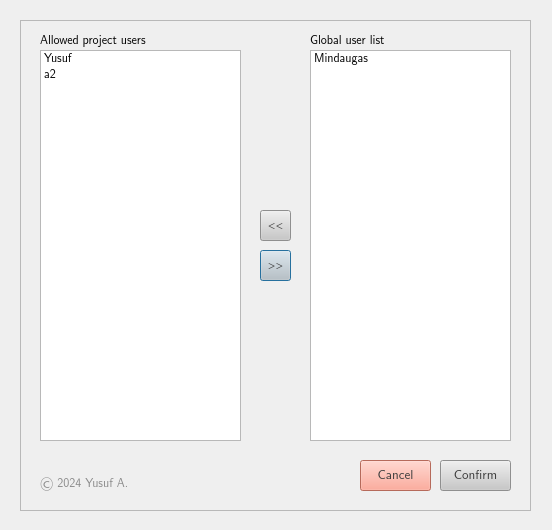
\includegraphics[width=0.8\textwidth]{modify-users}
		\caption{Modifying a project's user-list}
		\label{fig:modify-users}
	\end{figure}
	
	Modifying the project's user list is available to any authorised user, opening a new window (Fig. \ref{fig:modify-users})
	and allowing users to be moved from an available pool to the selected revision's user-list. The user cannot
	deselect himself or the project owner.
	
	Moving away from entry-related functionality, under \verb|Edit| $\rightarrow$ \verb|Preferences|, the user will
	be able to assign themselves a full name, which will be substituted on any form's occurrence of their name,
	this enables better tracking of changes.
	
	\newpage
	\subsubsection{Security}
	
	User passwords are hashed with \verb|SHA 256|, which is remarkably not a great hashing algorithm in itself,
	but it prevents trivial attempts to breach user security by a malicious actor. Primitive permission handling
	prevents a malicious actor from deleting projects which they are unauthorised to modify. Any prompts that
	involve creating a SQL query based off user input are processed through parametrised requests, enabling
	the ORM to perform library-level sanitisation.
	
	\subsubsection{Performance}
	
	The program uses an ORM (\verb|SQLAlchemy|) to allow the programmer to easily create and manage complex
	relationships between tables, this has a large impact on performance reduction because it allows the library
	to manage query-level optimisations through concepts such as lazy loading, and overall query reduction
	to solve $(n+1)$-style problems.
	
	Any relational DBMS is supported natively thanks to the ORM, and configuration is enabled through system
	environment variables.
	
	The UI is highly optimized due to \verb|Qt5|, which simplifies a lot of operations for the programmer, and 
	natively supports many complex tasks (such as date selection and tabling) that would otherwise be home
	-brewed.
	
	\subsection{Identifying five use-cases}
	
	\begin{figure}[h]
		\centering
		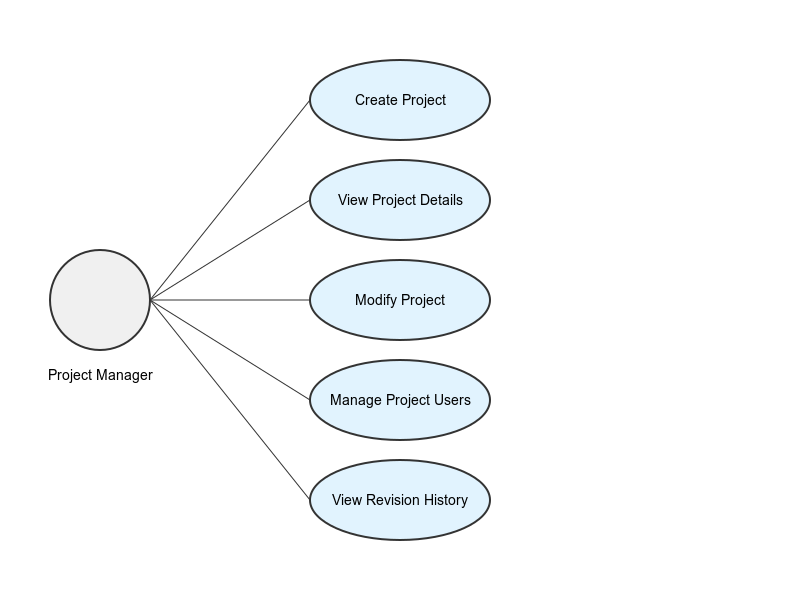
\includegraphics[width=0.8\textwidth]{use-cases}
		\caption{Use-case diagram}
		\label{fig:use-cases}
	\end{figure}
	
	\subsubsection{Creating a project}
	
	\begin{enumerate}
		\item Prerequisites
		\begin{enumerate}
			\item The user must have registered an account
			\item The user must be logged in
			\item The DBMS must be available
		\end{enumerate}
		\item Work flow
		\begin{enumerate}
			\item After the user has logged in, they navigate to \verb|Edit| $\rightarrow$ \verb|Create new entry|
					  through the action bar, displayed in Fig. \ref{fig:create-entry}
			\item The user may fill in any fields
			\item To finalise the project, the user presses the \verb|Create entry| button.
		\end{enumerate}
		\item The user is now assigned as the project owner, and is navigated to the \verb|View/edit entries|
				  form for their created project.
	\end{enumerate}
	
	\begin{figure}[h]
		\centering
		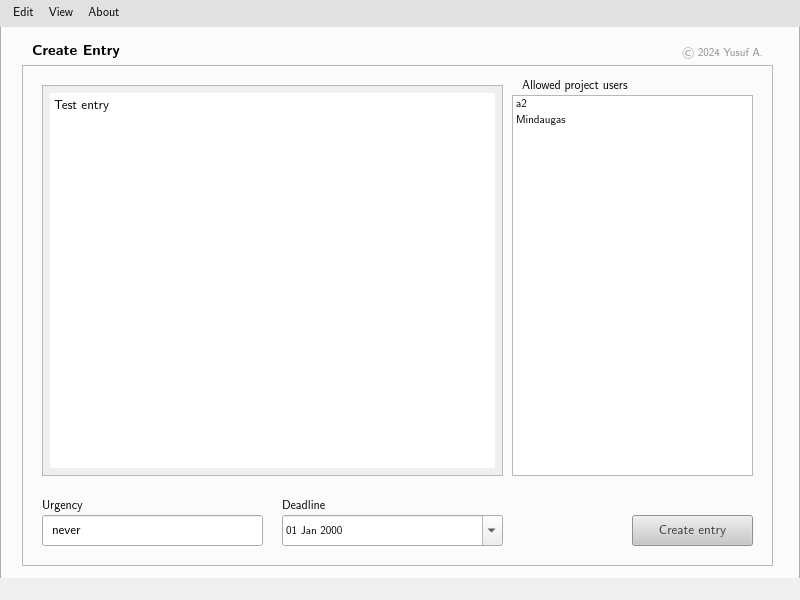
\includegraphics[width=0.8\textwidth]{create-entry}
		\caption{Create entry form}
		\label{fig:create-entry}
	\end{figure}
	
	\subsubsection{Viewing a project's details}

	\begin{enumerate}
		\item Prerequisites
		\begin{enumerate}
			\item The user must have registered an account
			\item The user must be logged in
			\item The project must exist 
			\item The DBMS must be available
		\end{enumerate}
		\item Work flow
		\begin{enumerate}
			\item After the user has logged in, they double-click on the project whose details they wish
					  to view
		\end{enumerate}
		\item The user may now view the project's latest details
	\end{enumerate}	
	
	\subsubsection{Modifying a project's details}
	
	\begin{enumerate}
		\item Prerequisites
		\begin{enumerate}
			\item The user must have registered an account
			\item The user must be logged in
			\item The project must exist 
			\item The user must be on the project's latest user list
			\item The DBMS must be available
		\end{enumerate}
		\item Work flow
		\begin{enumerate}
			\item After the user has logged in, they double-click on the project whose details they wish
					  to view
			\item The user may now click a revision under the \verb|Change history| table, and the system
					  will automatically load the revision
			\item The user must click the toggleable \verb|Edit| button to the active state
			\item The user may now edit any attribute of the project
			\item Once finished, the user must press the \verb|Confirm changes| button
		\end{enumerate}
		\item The changes made will be reflected in a new revision, which will be automatically selected
				  by the system.
	\end{enumerate}	
	
	\subsubsection{Managing a project's user list}
	
	\begin{enumerate}
		\item Prerequisites
		\begin{enumerate}
			\item The user must have registered an account
			\item The user must be logged in
			\item The project must exist 
			\item The user must be on the project's latest user list
			\item The DBMS must be available
		\end{enumerate}
		\item Work flow
		\begin{enumerate}
			\item After the user has logged in, they double-click on the project whose details they wish
			to view
			\item The user may now click a revision under the \verb|Change history| table, and the system
			will automatically load the revision
			\item The user must click the toggleable \verb|Edit| button to the active state
			\item The user must press the \verb|Modify project users| button, which will open a separate
					  dialog, as displayed in Fig. \ref{fig:modify-users}
			\item The user may select users to move to the \verb|Allowed project users| or to the
					  \verb|Global user list| as they wish.
			\item Once finished, the user must press the \verb|Confirm| button to reflect the changes on
					  the \verb|Edit entry| form.
			\item Once finished, the user must press the \verb|Confirm changes| button
		\end{enumerate}
		\item The changes made will be reflected in a new revision, which will be automatically selected
				  by the system.
	\end{enumerate}	
	
	\subsubsection{Viewing a specific project revision}

	\begin{enumerate}
		\item Prerequisites
		\begin{enumerate}
			\item The user must have registered an account
			\item The user must be logged in
			\item The project must exist 
			\item The DBMS must be available
		\end{enumerate}
		\item Work flow
		\begin{enumerate}
			\item After the user has logged in, they double-click on the project whose details they wish
					  to view
			\item The user may now click a revision under the \verb|Change history| table, and the system
					  will automatically load the revision
		\end{enumerate}
		\item The user may now view the revision's details
	\end{enumerate}	
	
	\newpage
	\section{Implementation}
	
	\newpage
	\section{Testing}
	
	If necessary, \verb|tests/test_database.py| is included to unit test the primary database mechanisms.
	including CRUD functionality, and more general function testing:
	
	\subsection{\texttt{test\_create\_user}}
	\vspace{1em}
	\begin{lstlisting}[language=Python]
		def test_create_users(self):
				with self.assertRaises(
					IntegrityError, msg="Username/password hash are non-optional"
				):
					self.db.users.create(username=None, password_hash=None)
				self.db.users.create(username="TestUser", password_hash="TestPassword")
				with self.assertRaises(
					IntegrityError, msg="Usernames cannot be repeated"
				):
					self.db.users.create(
						username="TestUser", password_hash="TestPassword"
					)
				self.db.users.create(
					username="TestUser1", password_hash="TestPassword"
				)
				users = self.db.users.get_all()
				self.assertTrue(len(users) == 2)
	\end{lstlisting}
	\vspace{1em}
	This tests against invalid user creation, duplication, and ensures the database commits changes.
	
	\subsection{\texttt{test\_create\_project}}
	\vspace{1em}
	\begin{lstlisting}[language=Python]
		def test_create_project(self):
			user1 = self.db.users.create(
				username="TestUser1", password_hash="TestPassword"
			)
			user2 = self.db.users.create(
				username="TestUser2", password_hash="TestPassword"
			)
			with self.assertRaises(
				IntegrityError, msg="Project cannot contain duplicate users"
			):
				proj1 = self.db.create_project(owner_id=user1, users=[user1])
			with self.assertRaises(
				IntegrityError, msg="Project cannot contain duplicate users"
			):
				proj1 = self.db.create_project(
					owner_id=user1, users=[user2, user2]
				)
			proj1 = self.db.create_project(owner_id=user1, users=[user2])
			self.assertEqual(proj1.owner_id, user1)
	\end{lstlisting}
	\vspace{1em}
	This tests creating a project. It ensures the interface does not allow inserting the owner as a
	project user, as this should be done automatically, and tests against regular double insertion.
	It also tests that the code correctly sets the owner user.
	
	\subsection{\texttt{test\_update\_project}}
	\vspace{1em}
	\begin{lstlisting}[language=Python]
		def test_update_project(self):
			user1 = self.db.users.create(
				username="TestUser1", password_hash="TestPassword"
			)
			user2 = self.db.users.create(
				username="TestUser2", password_hash="TestPassword"
			)
			proj1 = self.db.create_project(owner_id=user1, urgency="TestUrgency1")
			proj1.update(users=[user2], updated_by=user1)
			proj1.update(urgency="TestUrgency2", updated_by=user1)
			proj1.update(users=[], updated_by=user1)
			self.assertEqual(
				[*map(lambda p: len(proj1.get_users(p)), proj1.get_history())],
				[1, 2, 2, 1]
			)
			self.assertEqual(
				proj1.get_history()[2].urgency, "TestUrgency2"
			)
	\end{lstlisting}
	\vspace{1em}
	This tests to make sure revisions correctly store information across their creations.
	
	\subsection{\texttt{test\_delete\_revision}}
	\vspace{1em}
	\begin{lstlisting}[language=Python]
		def test_delete_revision(self):
			user1 = self.db.users.create(
				username="TestUser1", password_hash="TestPassword"
			)
			user2 = self.db.users.create(
				username="TestUser2", password_hash="TestPassword"
			)
			proj1 = self.db.create_project(owner_id=user1, urgency="TestUrgency1")
			proj1.update(urgency="TestUrgency2", updated_by=user1)
			proj1.update(urgency="TestUrgency3", users=[], updated_by=user1)
			self.assertEqual(proj1.get_latest().urgency, "TestUrgency3")
			proj1.remove(HistoricalProject.id == proj1.get_latest().id)
			self.assertEqual(proj1.get_latest().urgency, "TestUrgency2")
			proj1.remove(HistoricalProject.id == proj1.get_latest().id)
			self.assertEqual(proj1.get_latest().urgency, "TestUrgency1")
			with self.assertRaises(
				ValueError, msg="Can't remove the last project revision"
			):
				proj1.remove(HistoricalProject.id == proj1.get_latest().id)
	\end{lstlisting}
	This tests to make sure that revisions are stored in order when created, and that
	they are correctly deleted. This also tests for the case that the revision is the last one,
	and thus may not be deleted.
	
	\subsection{\texttt{test\_get\_user}}
	\vspace{1em}
	\begin{lstlisting}[language=Python]
		def test_get_user(self):
			user = self.db.users.create(username="TestUser", password_hash="TestHash")
			retrieved_user = self.db.users.get(User.id == user)
			self.assertEqual(retrieved_user.username, "TestUser")
	\end{lstlisting}
	\vspace{1em}
	This function test ensures that retrieving users works correctly.
	
	\subsection{\texttt{test\_update\_user}}
	\vspace{1em}
	\begin{lstlisting}[language=Python]
		def test_update_user(self):
			user = self.db.users.create(username="TestUser", password_hash="TestHash")
			self.db.users.update(user, full_name="Test Full Name")
			updated_user = self.db.users.get(User.id == user)
			self.assertEqual(updated_user.full_name, "Test Full Name")
	\end{lstlisting}
	\vspace{1em}
	This function tests ensures updating user details works correctly, this is relevant
	to the \verb|Preferences| tab.
	
	\subsection{\texttt{test\_get\_project}}
	\vspace{1em}
	\begin{lstlisting}[language=Python]
		def test_get_project(self):
			user = self.db.users.create(username="TestUser", password_hash="TestHash")
			project = self.db.create_project(owner_id=user, urgency="High")
			retrieved_project = self.db.get_project(ProjectEntry.id == project.id)
			self.assertEqual(retrieved_project.get_latest().urgency, "High")
	\end{lstlisting}
	\vspace{1em}
	This function test ensures retrieving projects works correctly.
	
	\subsection{\texttt{test\_get\_project\_users}}
	\vspace{1em}
	\begin{lstlisting}[language=Python]
		def test_get_project_users(self):
			user1 = self.db.users.create(username="User1", password_hash="Hash1")
			user2 = self.db.users.create(username="User2", password_hash="Hash2")
			project = self.db.create_project(owner_id=user1, users=[user2])
			project_users = project.get_users()
			self.assertEqual(len(project_users), 2)
			self.assertIn(user1, [u.id for u in project_users])
			self.assertIn(user2, [u.id for u in project_users])
	\end{lstlisting}
	\vspace{1em}
	This function test ensures the project users are assigned correctly.
	
	\subsection{\texttt{test\_get\_non\_existent\_project}}
	\vspace{1em}
	\begin{lstlisting}[language=Python]
		def test_get_non_existent_project(self):
			with self.assertRaises(IndexError):
				self.db.get_project(ProjectEntry.id == 9999)
	\end{lstlisting}
	\vspace{1em}
	This function test ensures that retrieving a project correctly errors when the
	\verb|expr| parameter is an invalid query.
	
\end{document}